\documentclass[dvipdfmx,cjk]{beamer}
\usepackage{mymacro}
\usepackage{tikz,here} % 図・コード
\usetikzlibrary{intersections,calc,arrows.meta,positioning}

\AtBeginDvi{\special{pdf:tounicode 90ms-RKSJ-UCS2}}
\AtBeginDvi{\special{pdf:tounicode EUC-UCS2}}

\setbeamertemplate{navigation symbols}{} %% 右下のアイコンを消す

%フレーム
%\usetheme{CambridgeUS}
%\usetheme{Boadilla}
\usetheme{Madrid}
%\usetheme{Antibes}
%\usetheme{Montpellier}
%\usetheme{Berkeley}
%\usetheme{Goettingen}
%\usetheme{Singapore}
%\usetheme{Szeged}

%色,フォント,内枠,外枠
%\usecolortheme{rose}
%\usecolortheme{albatross}
%\useoutertheme{shadow}                
\usefonttheme{professionalfonts}

%オプション
%\setbeamercovered{transparent}         %% 消えている文字をうっすらと表示する
\setbeamertemplate{theorems}[numbered] %% theorem 環境の冒頭に番号をつける

% 定理環境
\newtheorem{dfn}{定義}[section]
\newtheorem{thm}[dfn]{定理}
\newtheorem{exm}[dfn]{例}
\renewcommand{\proofname}{証明}

% マクロ
\def\Color{\textit{Color}}
\def\mix{\textit{mix}}
\def\red{\textit{red}}
\def\blu{\textit{blu}}
\def\yel{\textit{yel}}
\def\mix{\textit{mix}}
\def\colorYB{\textit{colorYB}}
\def\colorBYB{\textit{colorBYB}}
\def\colorYBBY{\textit{colorYBBY}}
\def\Cpos{\textit{Cpos}}
\def\WCT{\textit{WellColoredTriangle}}
\def\mixCut{\textit{mixCut}}
\def\AllRed{\textit{AllRed}}
\def\falseColor{\textit{falseColor}}
\def\Cexists{\textit{C\_exists}}
\def\Cuniq{\textit{C\_uniq}}
\def\Cmix{\textit{C\_mix}}
\def\Cpaint{\textit{C\_paint}}
\def\EvenA{\textit{EvenA}}
\def\EvenB{\textit{EvenB}}
\def\Even{\textit{Even}}
\def\ShortOddA{\textit{ShortOddA}}
\def\ShortOddB{\textit{ShortOddB}}
\def\ShortOddC{\textit{ShortOddC}}
\def\ShortOdd{\textit{ShortOdd}}
\def\LongOddA{\textit{LongOddA}}
\def\LongOddB{\textit{LongOddB}}
\def\LongOddC{\textit{LongOddC}}
\def\LongOdd{\textit{LongOdd}}

\begin{document}
\title[Coqによる三角形三色問題の証明]{Coqによる三角形三色問題の証明} 
\author{橋本 翔太 \and 木村 大輔 } %連名にする 発表者は下線を引くなどする
\institute{東邦大学大学院理学研究科 \and 東邦大学大学院理学研究科}
\date{September 1, 2, or 3, 2021} %日付は発表日に直すこと

% タイトルページ
\begin{frame}
  \titlepage
  \begin{center}
    {\footnotesize{日本ソフトウェア科学会第$38$回}}
  \end{center} 
\end{frame}

% 目次
\begin{frame}
\tableofcontents
\end{frame}

\section{本研究の概要}

\begin{frame}
  \frametitle{本研究の概要}
  \begin{block}{研究内容}
    三角形三色問題の解決するための定理証明をCoqで形式化する.
  \end{block}

  \vspace{10pt}
  三角形三色問題 $\cdots$ $3$色を用いてある規則に従って逆三角形に配置されたマスを塗り分けた図形に関する$2$つの問題
  \[
  % 9steps
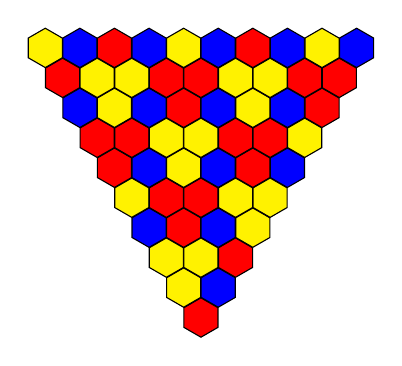
\begin{tikzpicture}[scale=0.25]
  %9段目
  \filldraw[fill=red] (0,0)--++(30:1)--++(90:1)--++(150:1)--++(210:1)--++(270:1)--cycle;
  %8段目
  \filldraw[fill=yellow,xshift={-25},yshift={25*sqrt(3)}] (0,0)--++(30:1)--++(90:1)--++(150:1)--++(210:1)--++(270:1)--cycle;
  \filldraw[fill=blue,xshift={25},yshift={25*sqrt(3)}] (0,0)--++(30:1)--++(90:1)--++(150:1)--++(210:1)--++(270:1)--cycle;
  %7段目
  \filldraw[fill=yellow,xshift={-25*2},yshift={25*sqrt(3)*2}] (0,0)--++(30:1)--++(90:1)--++(150:1)--++(210:1)--++(270:1)--cycle;
  \filldraw[fill=yellow,yshift={25*sqrt(3)*2}] (0,0)--++(30:1)--++(90:1)--++(150:1)--++(210:1)--++(270:1)--cycle;
  \filldraw[fill=red,xshift={25*2},yshift={25*sqrt(3)*2}] (0,0)--++(30:1)--++(90:1)--++(150:1)--++(210:1)--++(270:1)--cycle;
  %6段目
  \filldraw[fill=blue,xshift={-25*3},yshift={25*sqrt(3)*3}] (0,0)--++(30:1)--++(90:1)--++(150:1)--++(210:1)--++(270:1)--cycle;
  \filldraw[fill=red,xshift={-25},yshift={25*sqrt(3)*3}] (0,0)--++(30:1)--++(90:1)--++(150:1)--++(210:1)--++(270:1)--cycle;
  \filldraw[fill=blue,xshift={25},yshift={25*sqrt(3)*3}] (0,0)--++(30:1)--++(90:1)--++(150:1)--++(210:1)--++(270:1)--cycle;
  \filldraw[fill=yellow,xshift={25*3},yshift={25*sqrt(3)*3}] (0,0)--++(30:1)--++(90:1)--++(150:1)--++(210:1)--++(270:1)--cycle;
  %5段目
  \filldraw[fill=yellow,xshift={-25*4},yshift={25*sqrt(3)*4}] (0,0)--++(30:1)--++(90:1)--++(150:1)--++(210:1)--++(270:1)--cycle;
  \filldraw[fill=red,xshift={-25*2},yshift={25*sqrt(3)*4}] (0,0)--++(30:1)--++(90:1)--++(150:1)--++(210:1)--++(270:1)--cycle;
  \filldraw[fill=red,yshift={25*sqrt(3)*4}] (0,0)--++(30:1)--++(90:1)--++(150:1)--++(210:1)--++(270:1)--cycle;
  \filldraw[fill=yellow,xshift={25*2},yshift={25*sqrt(3)*4}] (0,0)--++(30:1)--++(90:1)--++(150:1)--++(210:1)--++(270:1)--cycle;
  \filldraw[fill=yellow,xshift={25*4},yshift={25*sqrt(3)*4}] (0,0)--++(30:1)--++(90:1)--++(150:1)--++(210:1)--++(270:1)--cycle;
  %4段目
  \filldraw[fill=red,xshift={-25*5},yshift={25*sqrt(3)*5}] (0,0)--++(30:1)--++(90:1)--++(150:1)--++(210:1)--++(270:1)--cycle;
  \filldraw[fill=blue,xshift={-25*3},yshift={25*sqrt(3)*5}] (0,0)--++(30:1)--++(90:1)--++(150:1)--++(210:1)--++(270:1)--cycle;
  \filldraw[fill=yellow,xshift={-25*1},yshift={25*sqrt(3)*5}] (0,0)--++(30:1)--++(90:1)--++(150:1)--++(210:1)--++(270:1)--cycle;
  \filldraw[fill=blue,xshift={25*1},yshift={25*sqrt(3)*5}] (0,0)--++(30:1)--++(90:1)--++(150:1)--++(210:1)--++(270:1)--cycle;
  \filldraw[fill=red,xshift={25*3},yshift={25*sqrt(3)*5}] (0,0)--++(30:1)--++(90:1)--++(150:1)--++(210:1)--++(270:1)--cycle;
  \filldraw[fill=blue,xshift={25*5},yshift={25*sqrt(3)*5}] (0,0)--++(30:1)--++(90:1)--++(150:1)--++(210:1)--++(270:1)--cycle;
  %3段目
  \filldraw[fill=red,xshift={-25*6},yshift={25*sqrt(3)*6}] (0,0)--++(30:1)--++(90:1)--++(150:1)--++(210:1)--++(270:1)--cycle;
  \filldraw[fill=red,xshift={-25*4},yshift={25*sqrt(3)*6}] (0,0)--++(30:1)--++(90:1)--++(150:1)--++(210:1)--++(270:1)--cycle;
  \filldraw[fill=yellow,xshift={-25*2},yshift={25*sqrt(3)*6}] (0,0)--++(30:1)--++(90:1)--++(150:1)--++(210:1)--++(270:1)--cycle;
  \filldraw[fill=yellow,yshift={25*sqrt(3)*6}] (0,0)--++(30:1)--++(90:1)--++(150:1)--++(210:1)--++(270:1)--cycle;
  \filldraw[fill=red,xshift={25*2},yshift={25*sqrt(3)*6}] (0,0)--++(30:1)--++(90:1)--++(150:1)--++(210:1)--++(270:1)--cycle;
  \filldraw[fill=red,xshift={25*4},yshift={25*sqrt(3)*6}] (0,0)--++(30:1)--++(90:1)--++(150:1)--++(210:1)--++(270:1)--cycle;
  \filldraw[fill=yellow,xshift={25*6},yshift={25*sqrt(3)*6}] (0,0)--++(30:1)--++(90:1)--++(150:1)--++(210:1)--++(270:1)--cycle;
  %2段目
  \filldraw[fill=blue,xshift={-25*7},yshift={25*sqrt(3)*7}] (0,0)--++(30:1)--++(90:1)--++(150:1)--++(210:1)--++(270:1)--cycle;
  \filldraw[fill=yellow,xshift={-25*5},yshift={25*sqrt(3)*7}] (0,0)--++(30:1)--++(90:1)--++(150:1)--++(210:1)--++(270:1)--cycle;
  \filldraw[fill=blue,xshift={-25*3},yshift={25*sqrt(3)*7}] (0,0)--++(30:1)--++(90:1)--++(150:1)--++(210:1)--++(270:1)--cycle;
  \filldraw[fill=red,xshift={-25*1},yshift={25*sqrt(3)*7}] (0,0)--++(30:1)--++(90:1)--++(150:1)--++(210:1)--++(270:1)--cycle;
  \filldraw[fill=blue,xshift={25*1},yshift={25*sqrt(3)*7}] (0,0)--++(30:1)--++(90:1)--++(150:1)--++(210:1)--++(270:1)--cycle;
  \filldraw[fill=yellow,xshift={25*3},yshift={25*sqrt(3)*7}] (0,0)--++(30:1)--++(90:1)--++(150:1)--++(210:1)--++(270:1)--cycle;
  \filldraw[fill=blue,xshift={25*5},yshift={25*sqrt(3)*7}] (0,0)--++(30:1)--++(90:1)--++(150:1)--++(210:1)--++(270:1)--cycle;
  \filldraw[fill=red,xshift={25*7},yshift={25*sqrt(3)*7}] (0,0)--++(30:1)--++(90:1)--++(150:1)--++(210:1)--++(270:1)--cycle;
  %1段目
  \filldraw[fill=red,xshift={-25*8},yshift={25*sqrt(3)*8}] (0,0)--++(30:1)--++(90:1)--++(150:1)--++(210:1)--++(270:1)--cycle;
  \filldraw[fill=yellow,xshift={-25*6},yshift={25*sqrt(3)*8}] (0,0)--++(30:1)--++(90:1)--++(150:1)--++(210:1)--++(270:1)--cycle;
  \filldraw[fill=yellow,xshift={-25*4},yshift={25*sqrt(3)*8}] (0,0)--++(30:1)--++(90:1)--++(150:1)--++(210:1)--++(270:1)--cycle;
  \filldraw[fill=red,xshift={-25*2},yshift={25*sqrt(3)*8}] (0,0)--++(30:1)--++(90:1)--++(150:1)--++(210:1)--++(270:1)--cycle;
  \filldraw[fill=red,yshift={25*sqrt(3)*8}] (0,0)--++(30:1)--++(90:1)--++(150:1)--++(210:1)--++(270:1)--cycle;
  \filldraw[fill=yellow,xshift={25*2},yshift={25*sqrt(3)*8}] (0,0)--++(30:1)--++(90:1)--++(150:1)--++(210:1)--++(270:1)--cycle;
  \filldraw[fill=yellow,xshift={25*4},yshift={25*sqrt(3)*8}] (0,0)--++(30:1)--++(90:1)--++(150:1)--++(210:1)--++(270:1)--cycle;
  \filldraw[fill=red,xshift={25*6},yshift={25*sqrt(3)*8}] (0,0)--++(30:1)--++(90:1)--++(150:1)--++(210:1)--++(270:1)--cycle;
  \filldraw[fill=red,xshift={25*8},yshift={25*sqrt(3)*8}] (0,0)--++(30:1)--++(90:1)--++(150:1)--++(210:1)--++(270:1)--cycle;
  %0段目
  \filldraw[fill=yellow,xshift={-25*9},yshift={25*sqrt(3)*9}] (0,0)--++(30:1)--++(90:1)--++(150:1)--++(210:1)--++(270:1)--cycle;
  \filldraw[fill=blue,xshift={-25*7},yshift={25*sqrt(3)*9}] (0,0)--++(30:1)--++(90:1)--++(150:1)--++(210:1)--++(270:1)--cycle;
  \filldraw[fill=red,xshift={-25*5},yshift={25*sqrt(3)*9}] (0,0)--++(30:1)--++(90:1)--++(150:1)--++(210:1)--++(270:1)--cycle;
  \filldraw[fill=blue,xshift={-25*3},yshift={25*sqrt(3)*9}] (0,0)--++(30:1)--++(90:1)--++(150:1)--++(210:1)--++(270:1)--cycle;
  \filldraw[fill=yellow,xshift={-25*1},yshift={25*sqrt(3)*9}] (0,0)--++(30:1)--++(90:1)--++(150:1)--++(210:1)--++(270:1)--cycle;
  \filldraw[fill=blue,xshift={25*1},yshift={25*sqrt(3)*9}] (0,0)--++(30:1)--++(90:1)--++(150:1)--++(210:1)--++(270:1)--cycle;
  \filldraw[fill=red,xshift={25*3},yshift={25*sqrt(3)*9}] (0,0)--++(30:1)--++(90:1)--++(150:1)--++(210:1)--++(270:1)--cycle;
  \filldraw[fill=blue,xshift={25*5},yshift={25*sqrt(3)*9}] (0,0)--++(30:1)--++(90:1)--++(150:1)--++(210:1)--++(270:1)--cycle;
  \filldraw[fill=yellow,xshift={25*7},yshift={25*sqrt(3)*9}] (0,0)--++(30:1)--++(90:1)--++(150:1)--++(210:1)--++(270:1)--cycle;
  \filldraw[fill=blue,xshift={25*9},yshift={25*sqrt(3)*9}] (0,0)--++(30:1)--++(90:1)--++(150:1)--++(210:1)--++(270:1)--cycle;
\end{tikzpicture}

  \text{段数}n=9\text{のとき}
  \]
\end{frame}

\begin{frame}
  \frametitle{三角形三色問題(規則)}
  次の$2$つ規則に従い逆三角形の上の段から下の段に向かって$3$色(赤,黄,青)で塗り分ける.

  \vspace{10pt}
  \begin{itemize}
  \item
    隣り合う色が同じとき同じ色をそれらと接する下の段のマスに塗る.
    \[
    % wellcolored
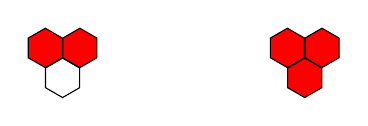
\begin{tikzpicture}[scale=0.25]
  %1段目
  \draw[xshift={-25*7},yshift={25*sqrt(3)*3}] (0,0)--++(30:1)--++(90:1)--++(150:1)--++(210:1)--++(270:1)--cycle;
  \filldraw[fill=red,xshift={25*7},yshift={25*sqrt(3)*3}] (0,0)--++(30:1)--++(90:1)--++(150:1)--++(210:1)--++(270:1)--cycle;
  %0段目
  \filldraw[fill=red,xshift={-25*6},yshift={25*sqrt(3)*4}] (0,0)--++(30:1)--++(90:1)--++(150:1)--++(210:1)--++(270:1)--cycle;
  \filldraw[fill=red,xshift={-25*8},yshift={25*sqrt(3)*4}] (0,0)--++(30:1)--++(90:1)--++(150:1)--++(210:1)--++(270:1)--cycle;
  \filldraw[fill=red,xshift={25*6},yshift={25*sqrt(3)*4}] (0,0)--++(30:1)--++(90:1)--++(150:1)--++(210:1)--++(270:1)--cycle;
  \filldraw[fill=red,xshift={25*8},yshift={25*sqrt(3)*4}] (0,0)--++(30:1)--++(90:1)--++(150:1)--++(210:1)--++(270:1)--cycle;
\end{tikzpicture}

    \]
  \item
    隣り合う色が異なるとき第三の色をそれらと接する下の段のマスに塗る.
    \[
    % wellcolored
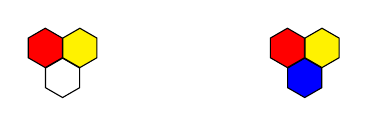
\begin{tikzpicture}[scale=0.25]
  %1段目
  \draw[xshift={-25*7},yshift={25*sqrt(3)*3}] (0,0)--++(30:1)--++(90:1)--++(150:1)--++(210:1)--++(270:1)--cycle;
  \filldraw[fill=blue,xshift={25*7},yshift={25*sqrt(3)*3}] (0,0)--++(30:1)--++(90:1)--++(150:1)--++(210:1)--++(270:1)--cycle;
  %0段目
  \filldraw[fill=yellow,xshift={-25*6},yshift={25*sqrt(3)*4}] (0,0)--++(30:1)--++(90:1)--++(150:1)--++(210:1)--++(270:1)--cycle;
  \filldraw[fill=red,xshift={-25*8},yshift={25*sqrt(3)*4}] (0,0)--++(30:1)--++(90:1)--++(150:1)--++(210:1)--++(270:1)--cycle;
  \filldraw[fill=red,xshift={25*6},yshift={25*sqrt(3)*4}] (0,0)--++(30:1)--++(90:1)--++(150:1)--++(210:1)--++(270:1)--cycle;
  \filldraw[fill=yellow,xshift={25*8},yshift={25*sqrt(3)*4}] (0,0)--++(30:1)--++(90:1)--++(150:1)--++(210:1)--++(270:1)--cycle;
\end{tikzpicture}

    \]
  \end{itemize}
\end{frame}

\begin{frame}
  \frametitle{三角形三色問題(問題)}
  \begin{block}{仮説}
    最上段をどのように塗っても逆三角形の端点の$3$マスの色はすべて同じ色 または すべて相異なる.
  \end{block}

  \vspace{10pt}
  三角形三色問題は次の$2$つである.
  \begin{block}{問題}
    \begin{itemize}
    \item
      $n=9$のとき仮説が成立することを証明せよ.
    \item
      $n=9$以外のときに仮説が成立する段数が存在するか調べ,
      存在するならば$n$の一般式を求めよ.
    \end{itemize}
  \end{block}
\end{frame}

\section{定義と公理}
\begin{frame}
  
\end{frame}
\section{十分条件の証明}
\begin{frame}
  
\end{frame}
\section{必要条件の証明}
\begin{frame}
  
\end{frame}
\section{まとめ}
\begin{frame}
  
\end{frame}
\end{document}

%memo
%1ページずつ伝えることを決める.→事前に紙に設計図を書いておく.
%スライドの1枚目は背景や目的を書く.
%(専門用語は簡単な説明をのせておけばよい→詳しい話はスライドの後半に載せる)
%この次のページは研究成果やできると何が良いのかを書く.

%公理化したのは工夫ポイント.(重要)

%定義,公理や証明は論文の切り貼りでも大丈夫→ただし,スライドの冒頭の説明がより伝わるようにすること.
